\section{Metamask}\label{section:metamask}
\subsection{Cos'è Metamask}
Metamask è un estensione per browser che ti permette di gestire il tuo wallet digitale di Ethereum e ti permette di inviare e ricevere Ether (Fantom in \projectName{}).
Metamask deve essere installato nel tuo browser per tutto il tempo che userai \projectName{}, senza di esso non potrai usare la nostra piattaforma.
\subsection{Installazione}
Dopo essere entrato in \projectName{}, controlla che Metamask sia installato, puoi farlo guardando se tra le estensioni in alto a destra è presente la sua icona.

    \begin{figure}[htbp]
        \centering
        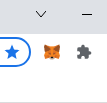
\includegraphics{immagini/metamask_installed.png}
        \caption{Metamask installato correttamente}
    \end{figure}   
 Se Metamask è installato correttamente, puoi procedere con l'utilizzo di \projectName, altrimenti consulta il video nella sezione sottostante (link video installazione metamask) e procedi con l'installazione.

\subsubsection{Configurazione}
Clicca l'icona di Metamask in alto a destra nel tuo browser e imposta il tuo wallet digitale Fantom seguendo le istruzioni.
Puoi creare un account nuovo, oppure importare uno già esistente tramite la frase iniziale di 12 parole che ti è stata precedentemente fornita.
